\documentclass{beamer}

\usepackage{amsmath}
\usepackage{amssymb}
\usepackage{amsthm}
\usepackage{tikz}
\usepackage{pgfplots}
\usepackage{graphicx}
\graphicspath{ {./img/} }

\usetheme{default}

\title{Inverting Vickrey}

\begin{document}

\begin{frame}{\titlepage}
  
\end{frame}

\begin{frame}{The setting}
  \only<-2>{
    We are assuming, as in (cite something) the cost function to be
    \begin{equation}
      \label{eq:cost}
      C(t_d) = \alpha tt(t_d) + \beta[t^*-t_d-tt(t_d)]^+ + \gamma[t_d+tt(t_d)-t^*]^+ 
    \end{equation}
  }
    \only<1>{
      where
      \begin{itemize}
      \item \(t^*\) is the desired arrival time
      \item \(\alpha\) is the value of time spent travelling
      \item \(\beta\) is the value of time spent waiting there
      \item \(\gamma\) is the value of time arriving late
      \item \(tt(t_d)\) is the expected (exogenous) travel time if leaving at time \(t_d\).
      \item \([x]^+ = \max(0, x)\)
      \end{itemize}
    }
    \only<2>{
      Without loss of generality, we can assume \(\alpha = 1\).

      Moreover, by defining the arrival time
      \begin{equation*}
        t_a = t_d + tt(t_d)
      \end{equation*}
      equation \eqref{eq:cost} becomes thus
    }
    \uncover<2->{
      \begin{equation}
        \label{eq:cost_ta}
        C(t_a) = tt_a(t_a) + \beta[t^*-t_a]^+ + \gamma[t_a-t^*]^+
      \end{equation}
    }
    \uncover<3>{
      We now assume the parameters \(\beta\), \(\gamma\) and the desired arrival times \(t^*\) to be normally distributed:
      \begin{itemize}
      \item \(\beta \sim \mathcal{N}(\mu_\beta, \sigma)\)
      \item \(\gamma \sim \mathcal{N}(\mu_\gamma, \sigma)\)
      \item \(t^* \sim \mathcal{N}(\mu_t, \sigma_t)\)
      \end{itemize}
    }
\end{frame}

\begin{frame}{Optimal arrival time samples}
  
  \begin{columns}
    \column{.4\linewidth}
      Drawing samples from these distributions, using a typical travel time function \(tt(t_a)\), the optima will be (in general) distributed as in the image,
      where the green and red zones roughly correspond to, respectively, early and late arrivals.

      Note that the x axis is random white noise, to better display the data distribution.
      
    \column{.6\linewidth}
    \centering
      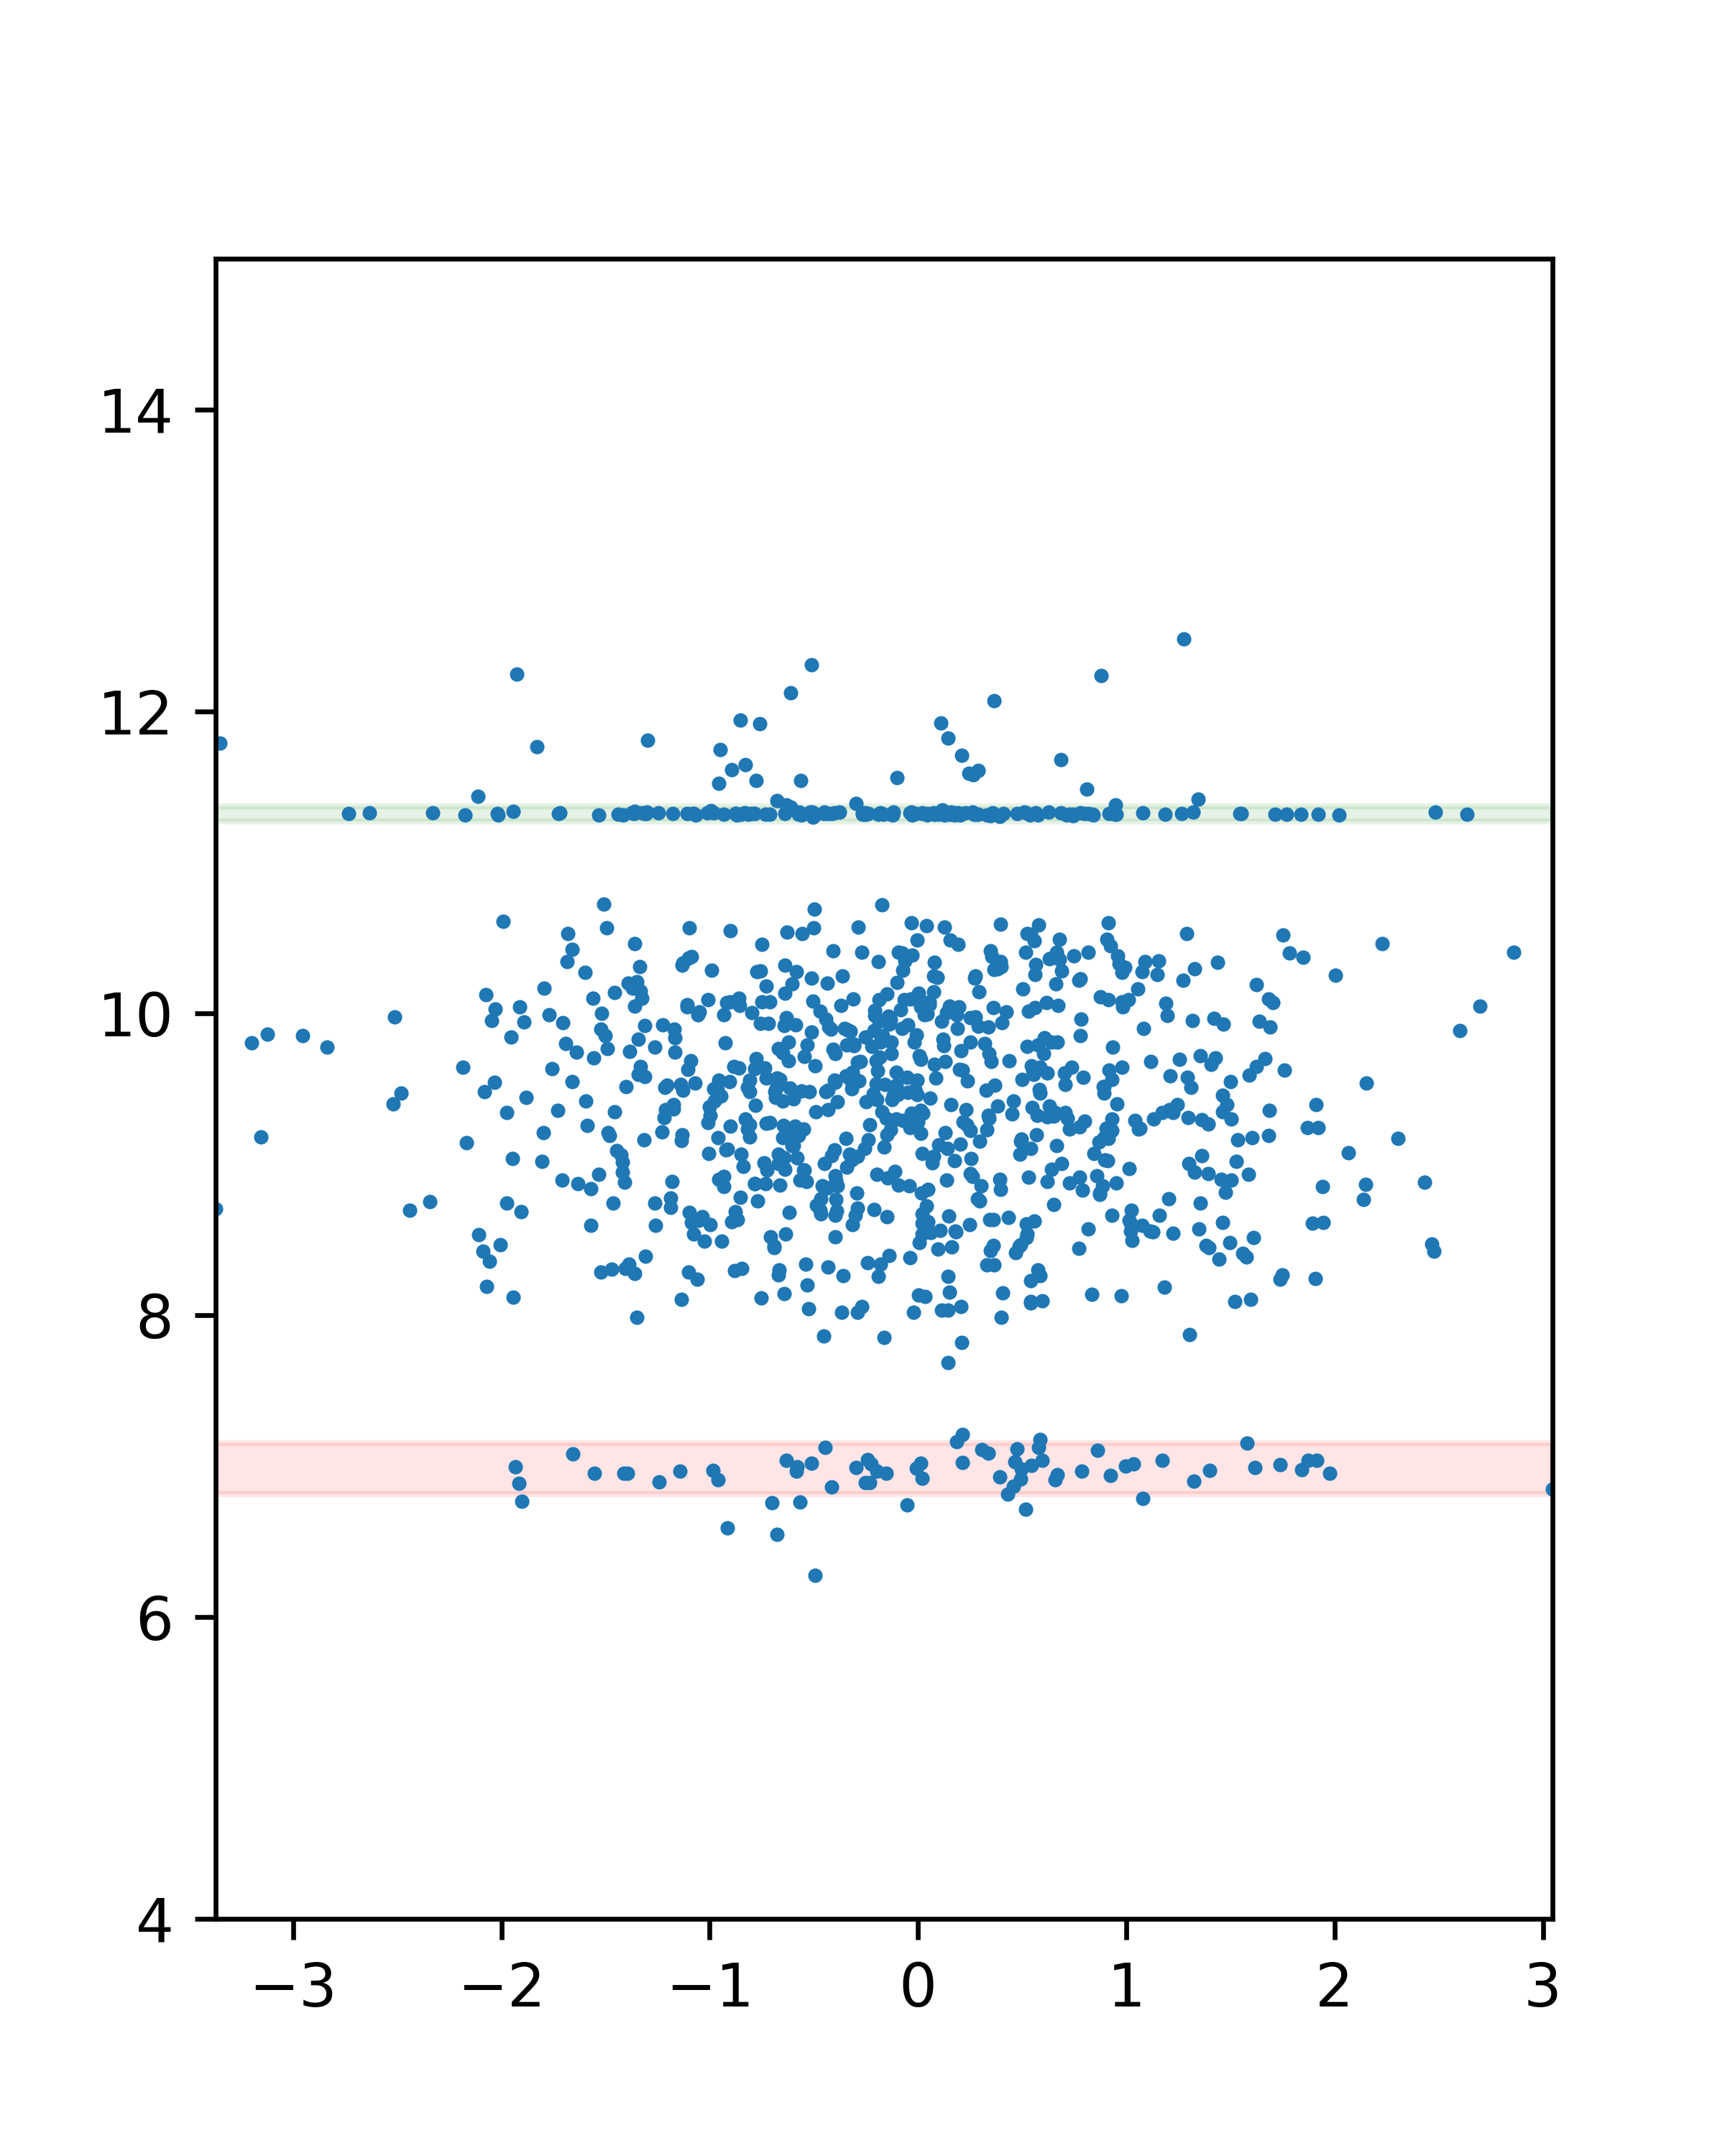
\includegraphics[width=\textwidth]{t_as}
  \end{columns}
\end{frame}

\begin{frame}{Optimal arrival time samples}
  As can be seen here, the early arrival are strictly correlated to the shape of the travel time function.
  \begin{center}
    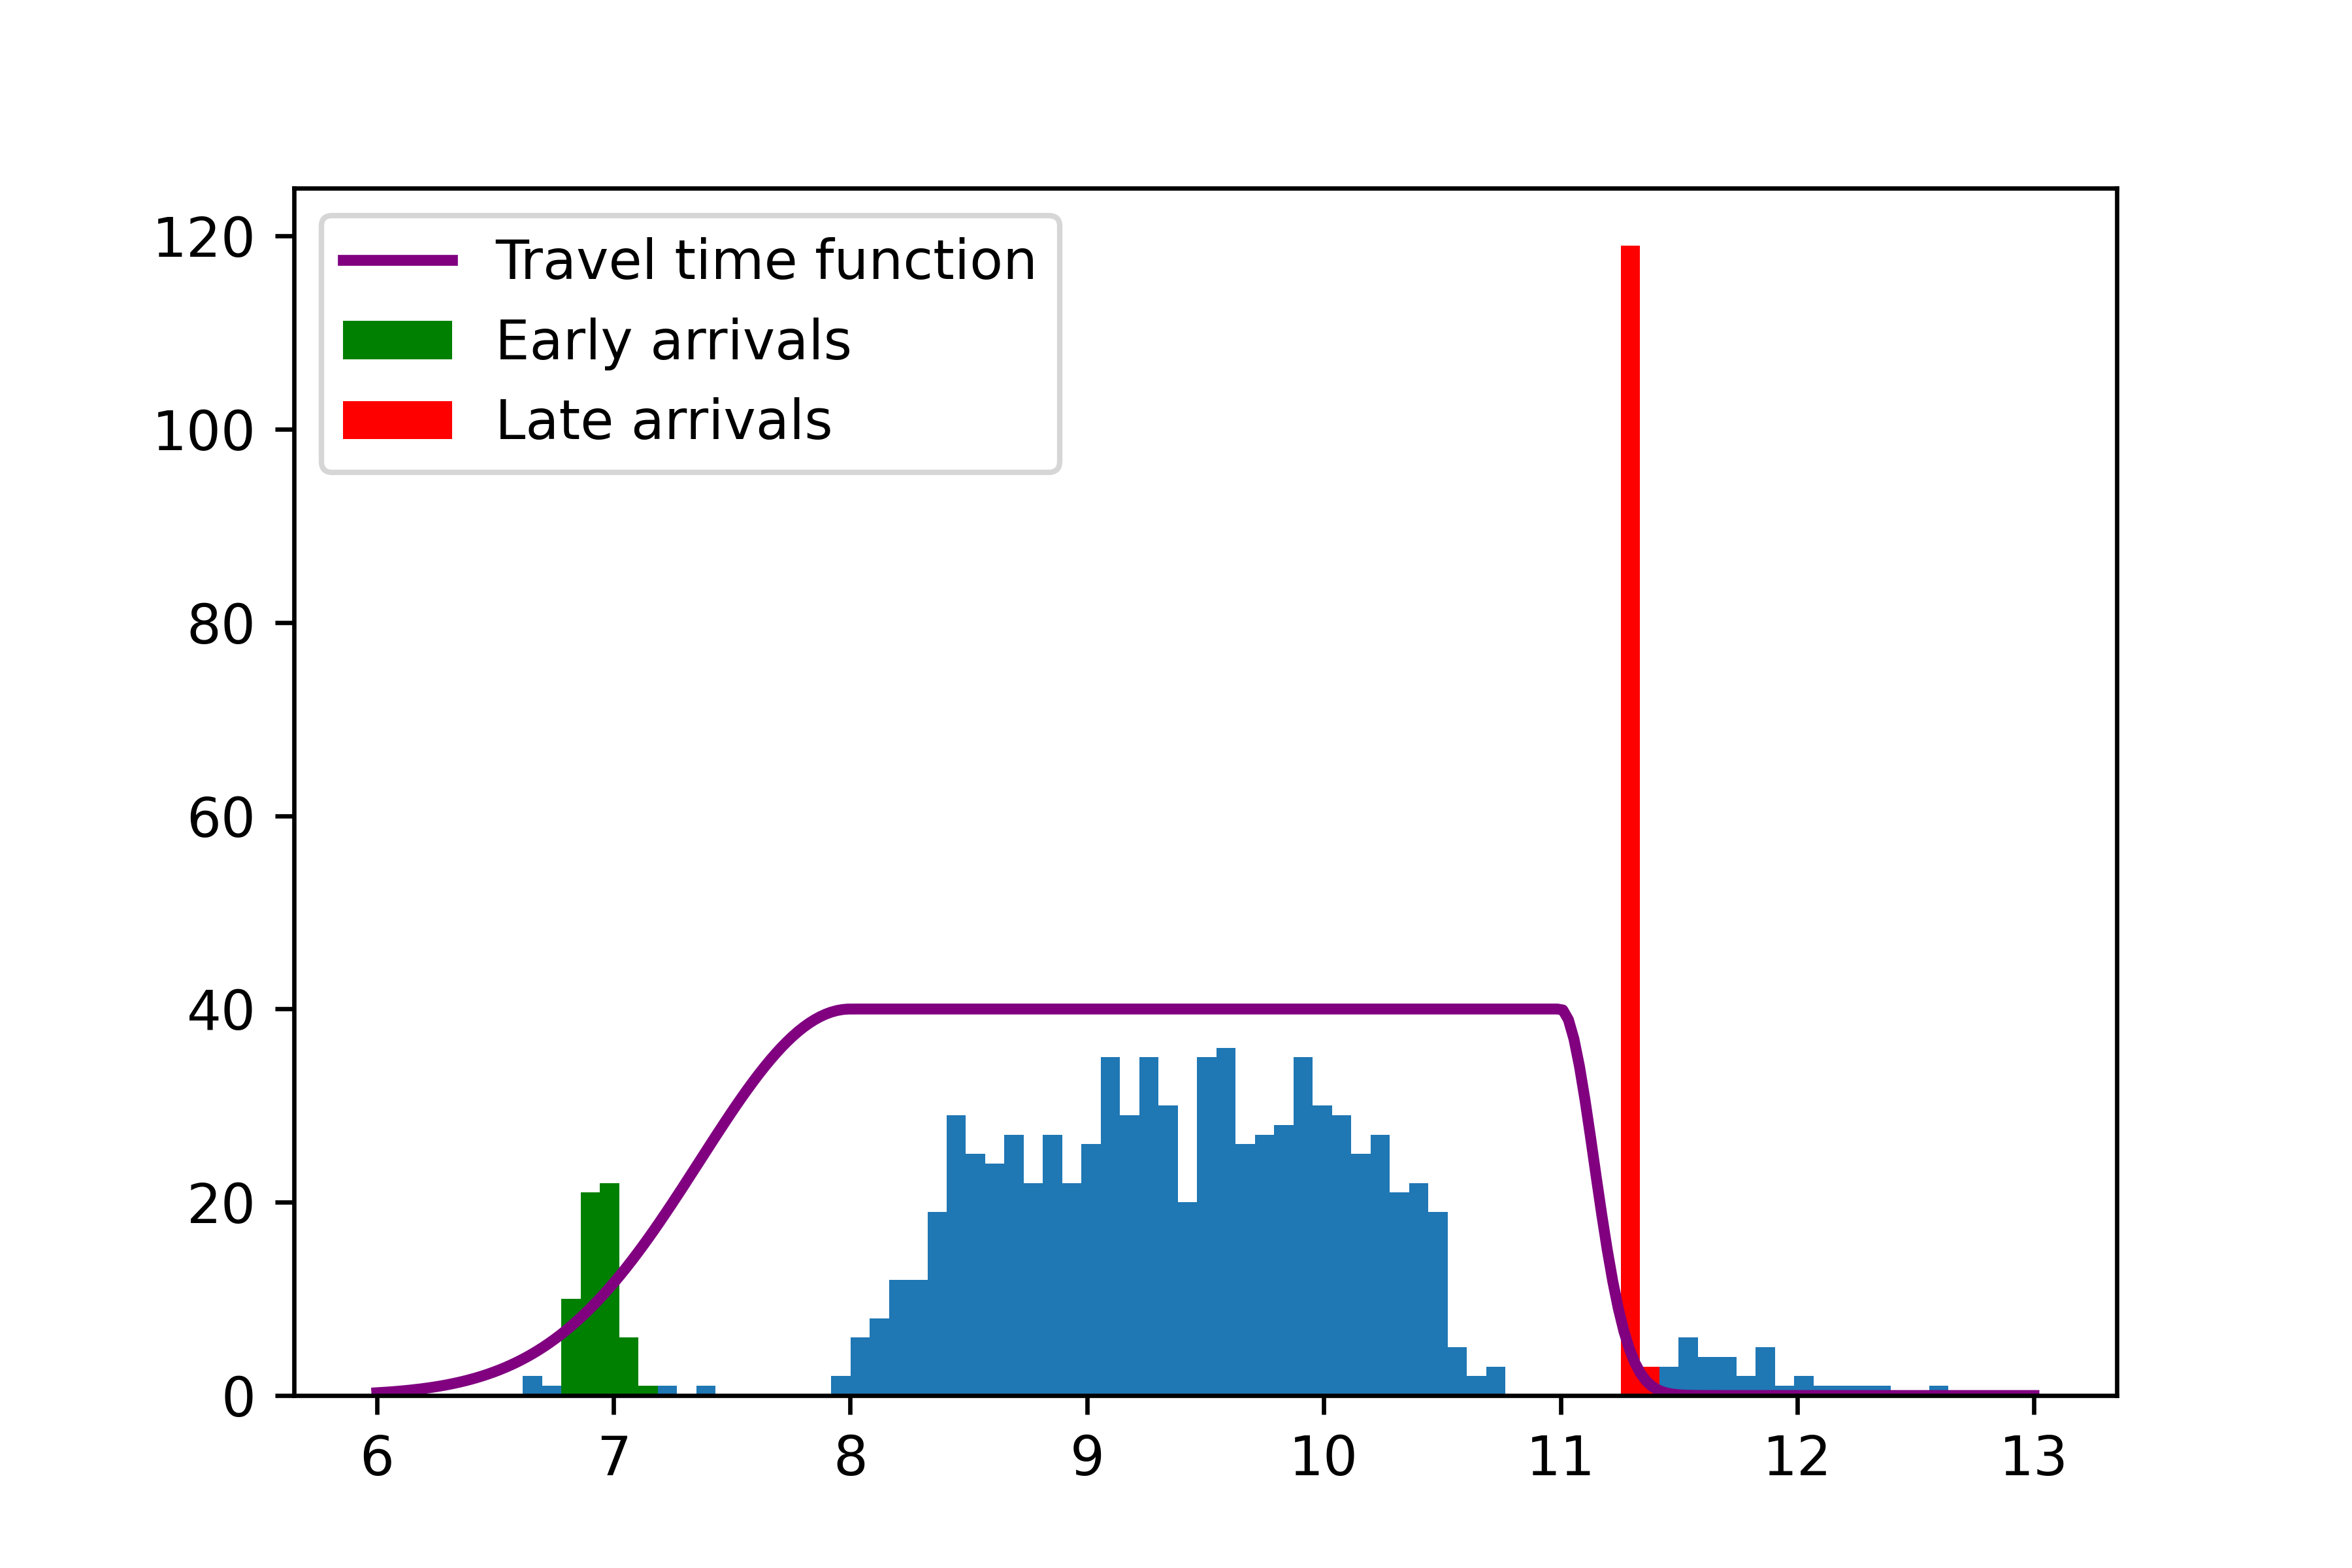
\includegraphics[width=\textwidth]{t_as_bins_tt}
  \end{center}
\end{frame}

\begin{frame}{Methodology}
  Our goal is thus finding, from the data about actual arrival times, the most likely values of mean and variances of the parameters \(\beta\) and \(\gamma\), on top of mean and variance for the desired arrival time \(t^*\).

  This was done by modelling the actual likelihood of each data point for a given parameter set
  \begin{equation*}
    \mathcal{L}(\mu_\beta, \mu_\gamma, \mu_t, \sigma, \sigma_t\ \vert\ T_a = t_a) =
  f_{T_a; \mu_\beta, \mu_\gamma, \mu_t, \sigma, \sigma_t}(t_a)
  \end{equation*}
  where \(f_{T_a; \theta}\) is the probability density function for the random variable \(T_a\),
  which describes the resulting optimal arrival time (namely, the one depicted in the plots above), given the parameters \(\theta\).
  
  Once the likelihood function is built, running an optimizer on the total likelihood of the dataset retrieves the true parameters for a given dataset.
\end{frame}

\begin{frame}{Building the likelihood function}
  To build the likelihood function, each point is assigned a probability of being an early, late or on time arrival.

  This is done by taking advantage of the key observation that early and late arrivals only occur when the desired arrival time \(t^*\) falls in certain zones defined by the parameters \(\alpha\) and \(\gamma\), namely the shaded zones in the plot below

  \begin{center}
    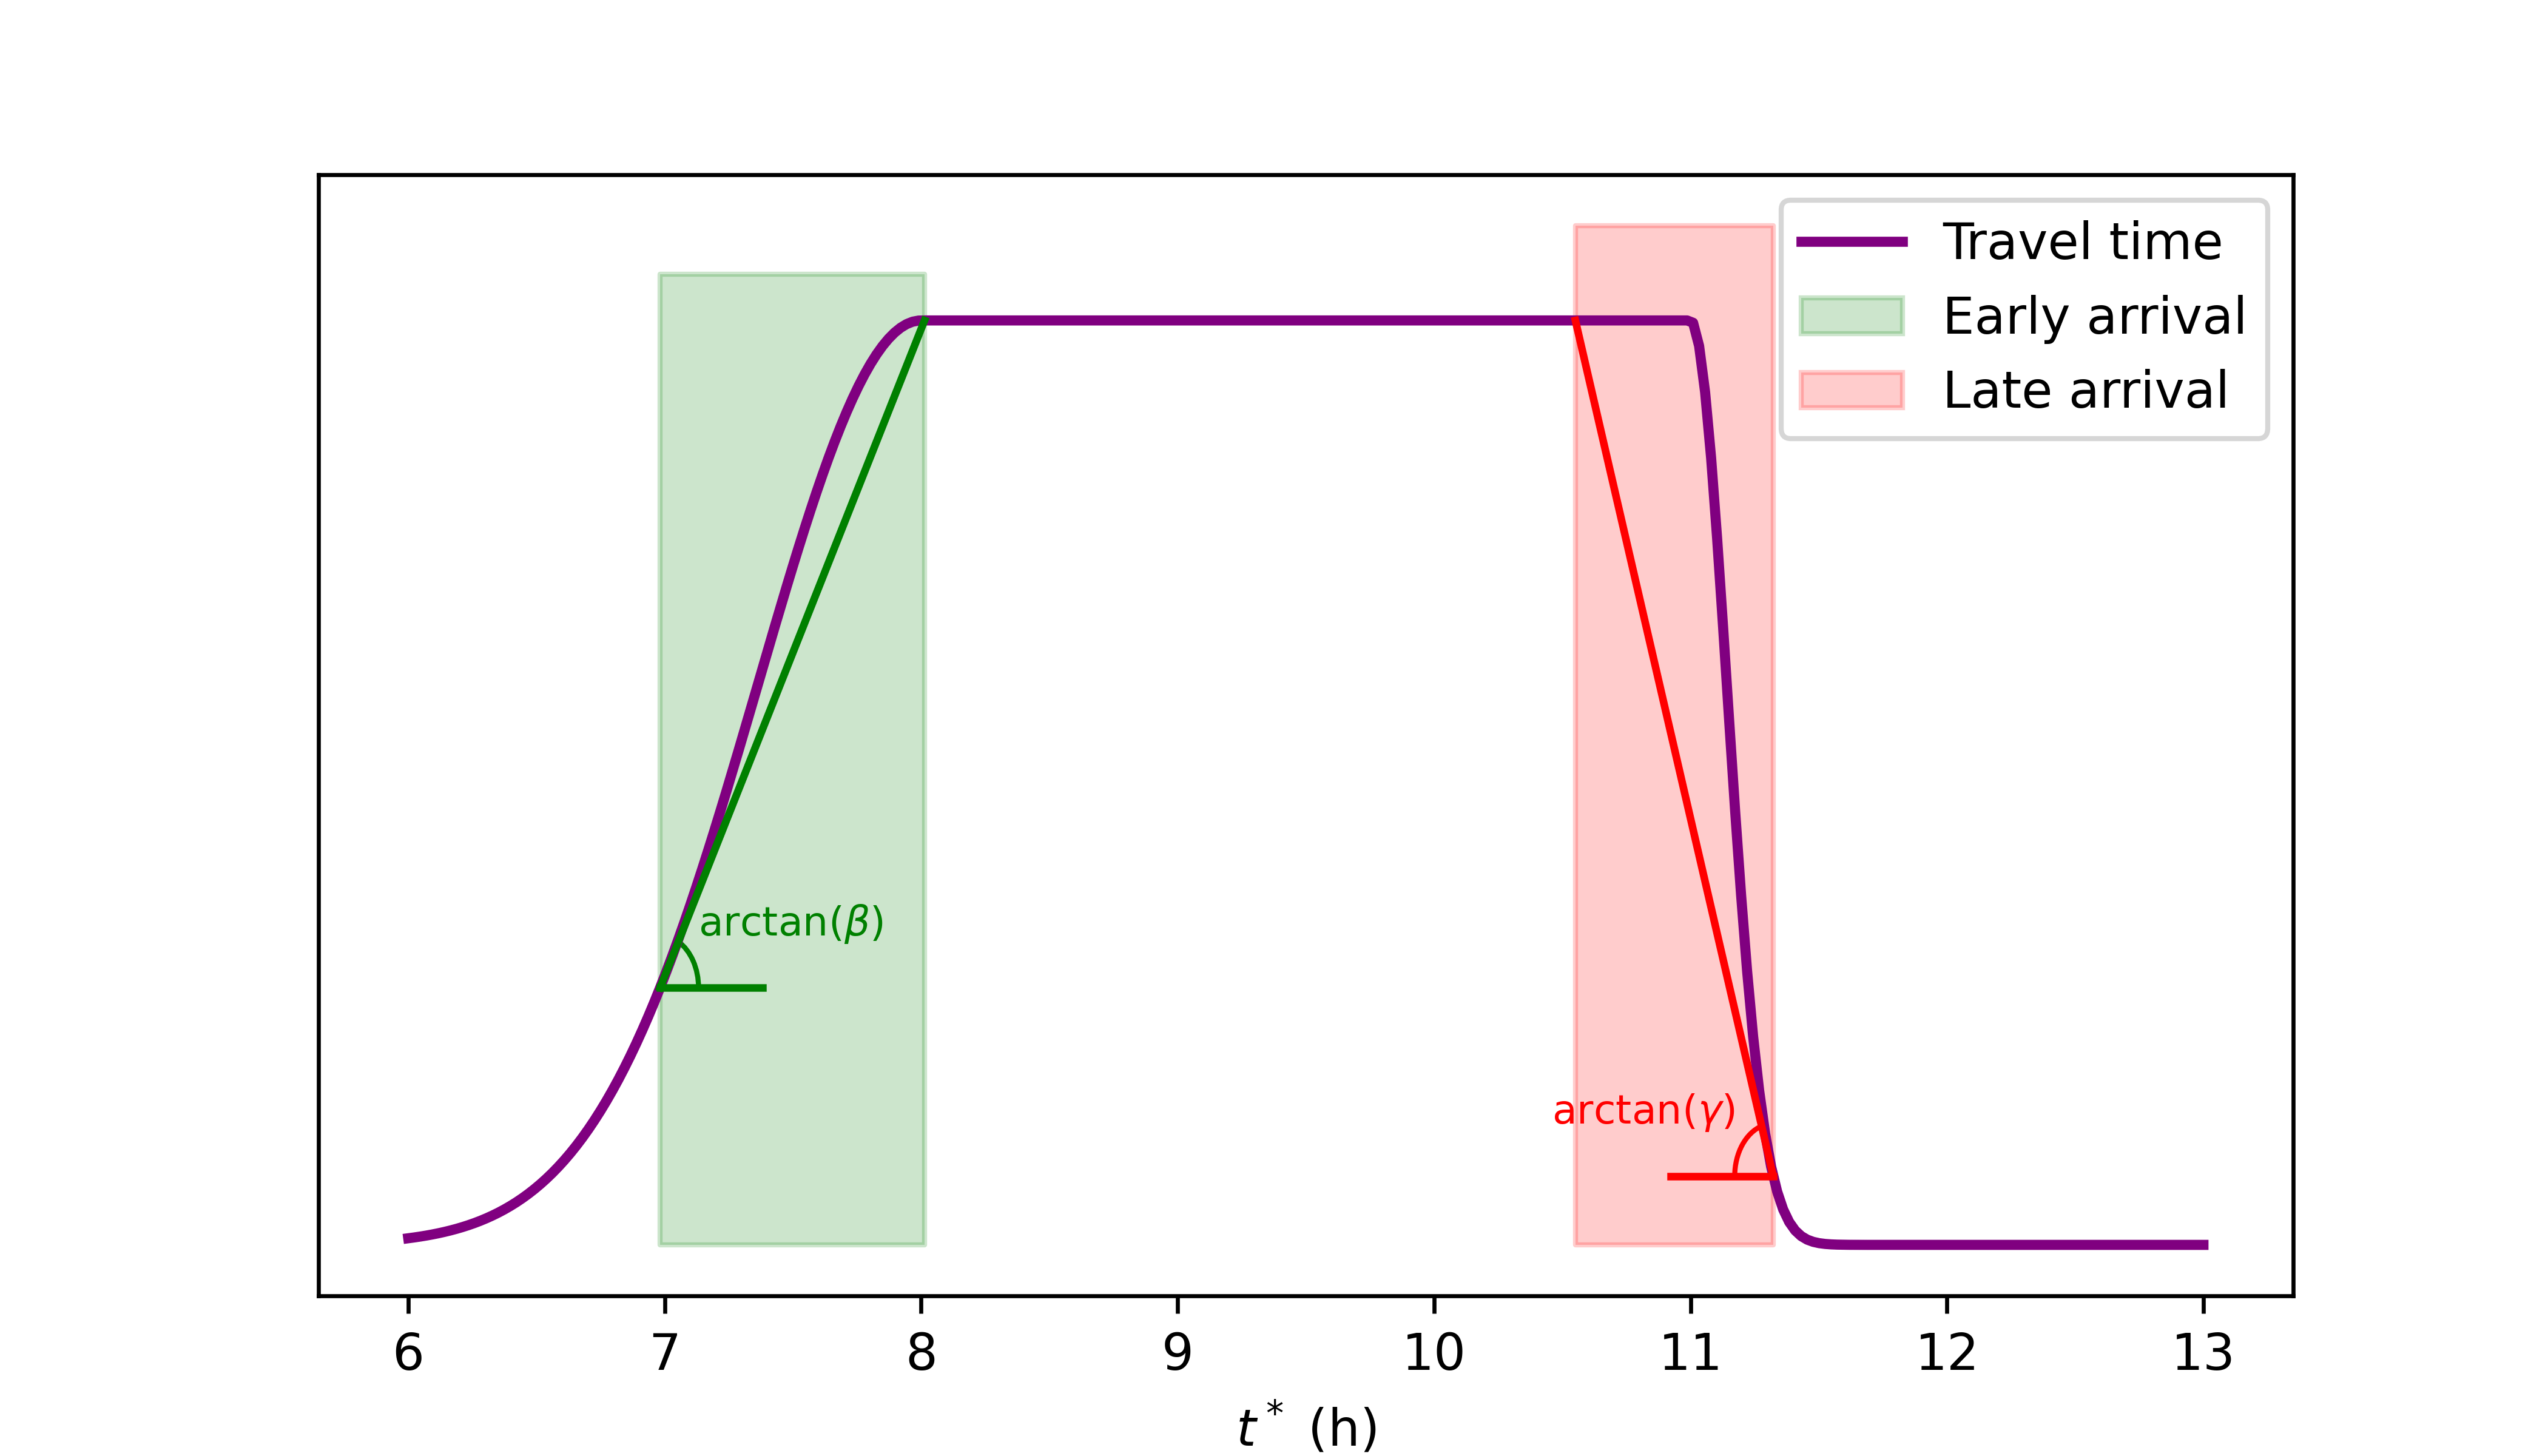
\includegraphics[width=.9\textwidth]{tt_early_late}
  \end{center}
\end{frame}
\end{document}

%%% Local Variables:
%%% mode: LaTeX
%%% TeX-master: t
%%% End:
